\documentclass[a4paper,10pt,twocolumn]{article}
\usepackage[utf8]{inputenc}
\usepackage[T1]{fontenc}
\usepackage[english]{babel}
\usepackage{mathpazo}
\usepackage[left=18mm,right=18mm,top=23mm,bottom=22mm,columnsep=7mm,headheight=13pt,headsep=7mm]{geometry}
\usepackage{graphicx}
\graphicspath{{images/}}
\usepackage{float}
\usepackage{amsmath,amssymb}
\usepackage{url}
\usepackage{tikz}
\usepackage{booktabs,multirow}
\usepackage{balance}
\usepackage{microtype}
\usepackage{titlesec}
\usepackage[font=small,labelfont=sc,labelsep=colon]{caption}
\usepackage{fancyhdr}
\pagestyle{fancy}
\fancyhf{}
\fancyhead[L]{\small Fuzzy charging control for lithium-ion batteries}
\fancyhead[R]{\small\thepage}
\renewcommand{\headrulewidth}{0pt}
\titleformat{\section}{\normalfont\fontsize{12}{14}\selectfont\bfseries}{\thesection.}{0.5em}{}
\titlespacing*{\section}{0pt}{12pt plus 2pt minus 1pt}{6pt}
\titleformat{\subsection}[runin]{\normalfont\itshape}{\thesubsection.}{0.5em}{}[.]
\titlespacing*{\subsection}{0pt}{9pt plus 2pt minus 1pt}{0.6em}
\titleformat{\subsubsection}[runin]{\normalfont\itshape}{\thesubsubsection.}{0.5em}{}[.]
\titlespacing*{\subsubsection}{0pt}{8pt}{0.6em}
\setlength{\parindent}{1.5em}
\setlength{\textfloatsep}{12pt plus 2pt minus 2pt}
\setlength{\floatsep}{10pt plus 2pt minus 2pt}
\renewenvironment{abstract}{\par\begingroup\small\noindent\ignorespaces}{\par\endgroup}
\makeatletter
\newcommand{\portadaarticulo}{%
  {\raggedright\fontsize{18}{21}\selectfont\bfseries\@title\par}%
  \vspace{14pt}%
  {\normalsize\bfseries Leo Nick Condori Gallegos\par}%
  \vspace{5pt}%
  {\small\itshape School of Electronic Engineering,\\
  Universidad Nacional de San Agustín de Arequipa, Arequipa, Peru\par}%
  \vspace{4pt}%
  {\small\texttt{lcondoriga@unsa.edu.pe}\par}\vspace{12pt}%
}
\makeatother
\usepackage[hidelinks]{hyperref}
\usetikzlibrary{arrows.meta,positioning,shapes.geometric,calc}
\setlength{\emergencystretch}{2em}
\raggedbottom
\setcounter{topnumber}{3}
\renewcommand{\topfraction}{0.90}
\renewcommand{\textfraction}{0.10}
\renewcommand{\floatpagefraction}{0.78}
\setlength{\parskip}{0pt}
\renewcommand{\figurename}{Figure}
\renewcommand{\tablename}{Table}
% Generated by MATLAB build_paper_assets.m.
\newcommand{\TimeCC}{3203}
\newcommand{\TimeFZ}{6761}
\newcommand{\PeakIFZ}{1.876}
\newcommand{\RiseCC}{1.60}
\newcommand{\RiseFZ}{0.47}
\newcommand{\StaticCurrent}{1.627}
\newcommand{\TrackingError}{0}
\newcommand{\ExtraTimeFZ}{3558}
\newcommand{\RelativeExtraFZ}{111.1}
\newcommand{\ExtendedCCPeak}{1.60}
\newcommand{\ExtendedFZPeak}{0.47}
\newcommand{\ExtendedCCPeakTime}{3207}
\newcommand{\ExtendedFZPeakTime}{1320}
\newcommand{\ExtendedCCStop}{3711}
\newcommand{\ExtendedFZStop}{6874}
\newcommand{\ExtendedCCSOC}{99.00}
\newcommand{\ExtendedFZSOC}{99.01}
\newcommand{\ExtendedCCVoltage}{4.2051}
\newcommand{\ExtendedFZVoltage}{4.2834}
\newcommand{\ExtendedCCCurrent}{2.2000}
\newcommand{\ExtendedFZCurrent}{1.8759}
\newcommand{\CCSolverChange}{0.0}
\newcommand{\FZSolverChange}{0.0}
\newcommand{\CCSampleChange}{-0.5}
\newcommand{\FZSampleChange}{0.0}
\newcommand{\OutputMFs}{%
VS & $(3.080,3.080,3.385)$ & $(0.000,0.000,0.305)$ & $(0.2047,0.7058,1.1263)$ \\
S & $(3.080,3.385,3.690)$ & $(0.000,0.305,0.610)$ & $(0.7684,1.0726,1.4842)$ \\
M & $(3.385,3.690,3.995)$ & $(0.305,0.610,0.915)$ & $(1.1263,1.3411,1.8421)$ \\
L & $(3.690,3.995,4.300)$ & $(0.610,0.915,1.220)$ & $(1.4842,1.7347,2.2000)$ \\
VL & $(3.995,4.300,4.300)$ & $(0.915,1.220,1.220)$ & $(1.8421,2.0926,2.5579)$ \\
}
\newcommand{\NominalRows}{%
CC--CV & 3203 & 2.200 & 91.47 & 1.60 \\
Mamdani & 6761 & 1.876 & 97.83 & 0.47 \\
}
\newcommand{\CurrentRows}{%
1.10 & 6827 & 7119 & 1.100 \\
1.50 & 4938 & 6788 & 1.500 \\
1.80 & 4049 & 6762 & 1.800 \\
2.20 & 3203 & 6761 & 1.876 \\
}
\newcommand{\SOCRows}{%
2.5, 2.5, 2.5, 2.5 & 3203 & 6761 & 0 & 0 & all/all \\
20, 20, 20, 20 & 2573 & 5798 & 0 & 0 & all/all \\
40, 40, 40, 40 & 1853 & 4417 & 0 & 0 & all/all \\
15, 18, 22, 25 & 2393 & 5475 & 58 & 126 & BV4/BV4 \\
5, 15, 25, 35 & 2033 & 4779 & 109 & 160 & BV4/BV4 \\
35, 25, 15, 5 & 2033 & 4779 & 109 & 160 & BV1/BV1 \\
}
\newcommand{\ThermalRows}{%
40.5 & 20 & 1.60 & 3207 & 0.47 & 1320 \\
36.0 & 10 & 0.81 & 3204 & 0.30 & 708 \\
36.0 & 30 & 2.32 & 3219 & 0.65 & 1632 \\
50.0 & 10 & 0.81 & 3204 & 0.27 & 916 \\
50.0 & 30 & 2.16 & 3244 & 0.59 & 2817 \\
}
\newcommand{\OutputSensitivityRows}{%
2.5, 2.5, 2.5, 2.5 & 6761 & 7721 & 0 & 0 \\
20, 20, 20, 20 & 5798 & 6592 & 0 & 0 \\
5, 15, 25, 35 & 4779 & 5429 & 160 & 163 \\
}
\newcommand{\OutputDeltaBaseline}{+960}
\newcommand{\OutputDeltaMean}{+794}
\newcommand{\OutputDeltaSpread}{+650}

% Generated from the benchmark and Validacion_Eisto CSV files.
\newcommand{\LateLowCap}{4.3}
\newcommand{\TimeNinetyCC}{3150}
\newcommand{\VoltNinetyCC}{4.188}
\newcommand{\RiseNinetyCC}{1.59}
\newcommand{\TimeNinetyFZ}{6120}
\newcommand{\VoltNinetyFZ}{4.091}
\newcommand{\RiseNinetyFZ}{0.47}
\newcommand{\LateNinety}{94.3}
\newcommand{\EistoRefV}{113.5}
\newcommand{\EistoSimV}{116.8}
\newcommand{\EistoAbsGapV}{3.3}
\newcommand{\EistoRefI}{109.7}
\newcommand{\EistoSimI}{116.8}
\newcommand{\EistoVoltMAE}{123.9}
\newcommand{\EistoCurrentMAE}{56.3}
\newcommand{\EistoProgressMAE}{1.6}

\title{Comparison of CC--CV and Mamdani Charging in Series-Connected Lithium-Ion Cells with Electrical Analysis and Thermal Estimation}
\author{Leo Nick Condori Gallegos}
\date{}
\begin{document}
\twocolumn[{%
\begin{minipage}{\textwidth}
\portadaarticulo
\begin{abstract}
\textbf{Abstract.}
This simulation study compares constant-current--constant-voltage (CC--CV) charging with a nominal Mamdani controller for four series-connected $2.2\,\mathrm{Ah}$ lithium-ion cells. From a uniform initial state of charge (SOC) of $2.5\,\%$, Mamdani took \RelativeExtraFZ\% longer than CC--CV to reach the first per-cell threshold of $4.2\,\mathrm{V}$ under a $2.2\,\mathrm{A}$ current limit. The difference fell to \LateLowCap\% under a $1.1\,\mathrm{A}$ limit. At the common endpoint of $90\,\%$ SOC and the nominal current limit, CC--CV and Mamdani took \TimeNinetyCC\ and \TimeNinetyFZ\,s, with peak estimated temperature rises of \RiseNinetyCC\ and \RiseNinetyFZ\,K, respectively. The sensitivity analysis varied the applied-current ceiling, Mamdani output range, initial SOC, and thermal parameters. A separate cell-level comparison against the published $1.1\,\mathrm{A}$ Eisto profile quantified the agreement in voltage, current, and relative charge.
\end{abstract}
\vspace{5pt}
{\small\noindent\textbf{Keywords.} Lithium-ion battery, CC--CV, Mamdani inference, series cells, thermal estimation.\par}
\end{minipage}
\vspace{12pt}
}]

\section{Introduction}
\label{sec:intro}
The charging current influences lithium-ion cell terminal voltage through the resistive and polarization responses. It also sets the magnitude of Joule heat generation. In a series string the same current flows through all cells, and a cell with a higher initial state of charge can reach its voltage limit while the remaining cells are still below it. A comparison based on the first cell to reach its limit can therefore yield a different result from a comparison based on average SOC or full charging time.

Constant-current--constant-voltage (CC--CV) charging is the reference strategy in this study because it is a conventional charging protocol and its constant-current stage gives a well-defined benchmark up to the transition voltage~\cite{tomaszewska2019,ghaeminezhad2022}. Fuzzy charging can vary the current throughout the run using a rule base. Ali et al.~\cite{ali2018} studied fuzzy charging with thermal feedback and a laboratory implementation. Table~\ref{tab:literature} compares five more recent approaches.

\begin{table*}[t]
\centering
\small
\caption{Lithium-ion charging strategies in recent studies.}
\label{tab:literature}
\begin{tabular}{@{}p{0.25\textwidth}p{0.24\textwidth}p{0.16\textwidth}p{0.25\textwidth}@{}}
\toprule
Study and strategy & Control variables or parameters & Evaluation & Reported metrics \\
\midrule
Károlyi et al.~\cite{karolyi2022}, fuzzy control tuned by a genetic algorithm &
Cell temperature and FIS parameters &
Equivalent circuit model &
Charging time and temperature \\
Nizam et al.~\cite{nizam2022}, CC followed by fuzzy control &
Voltage for the transition, temperature and its variation for fuzzy control &
Prototype tests &
Charging time relative to CC--CV \\
Kalk et al.~\cite{kalk2024}, multistage constant current &
Estimated SOC and current in each stage &
Cell tests &
Time from $0$ to $80\,\%$ SOC \\
Manjunatha et al.~\cite{perfil2024}, predefined current profile &
Applied current profile &
Tests on C/NCA cells &
Time to $80\,\%$ SOC and temperature rise \\
Sardahi et al.~\cite{sardahi2026}, Mamdani with multiobjective tuning &
Minimum cell voltage and voltage spread &
Simulink simulation &
Time to $95\,\%$ SOC, peak temperature, and current-stress index \\
\bottomrule
\end{tabular}
\end{table*}

Studies in Table~\ref{tab:literature} use different cells, feedback signals, and endpoints. Their reported charging times do not directly answer the question considered here. Under a shared current limit and a common four-cell model, how do CC--CV and a voltage-based Mamdani policy differ in time to the first cell reaching $4.2\,\mathrm{V}$, voltage dispersion at that event, and estimated heating? Which differences persist when the applied-current ceiling, the Mamdani output range, and the initial SOC profile are varied? The benchmark holds the electrical model and endpoints fixed, makes the adopted rule policy~\cite{chuang} explicit, and relates the electrical and thermal results to the applied current.

The central finding is that the time penalty associated with the Mamdani profile depends strongly on the current ceiling. Its time to the first $4.2\,\mathrm{V}$ crossing was \RelativeExtraFZ\% longer at the nominal ceiling of $2.2\,\mathrm{A}$ and \LateLowCap\% longer at $1.1\,\mathrm{A}$. A second comparison at a common SOC separates this timing effect from differences in stored charge at the voltage event. A manufacturer-referenced cell analysis also quantifies the agreement that can be established from the published charging profile.

\section{Charging strategies and battery model}
\label{sec:model}
\subsection{CC--CV operation}
During CC, the source applies the prescribed current until the monitored terminal voltage reaches its transition criterion. During CV, the source regulates the voltage and the charging current tapers. The CV interval extends the full charging process beyond the first threshold crossing. The manufacturer's standard charge specifies a $44\,\mathrm{mA}$ termination current~\cite{eisto2200}. Figure~\ref{fig:charging_curve} shows the manufacturer reference for a single cell charged at $0.5C$.

\begin{figure}[htbp]
\centering
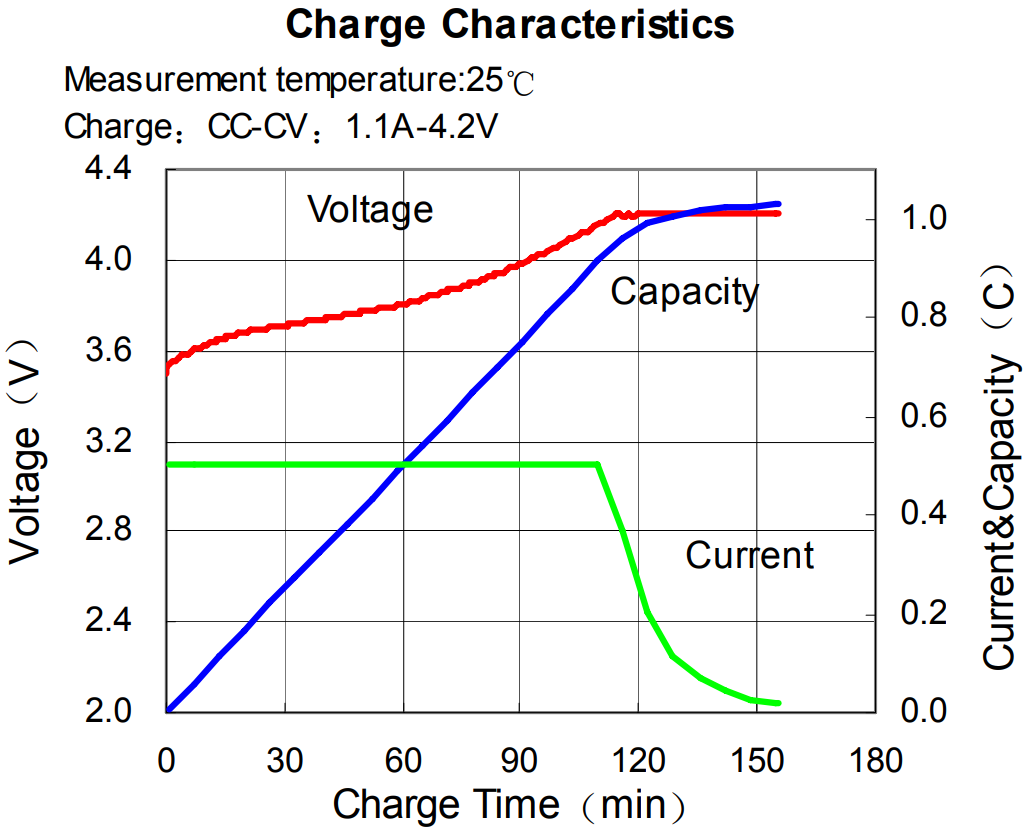
\includegraphics[width=\linewidth]{eisto_charge_characteristics.png}
\caption{Eisto ICR18650 charge characteristics at $25\,^{\circ}\mathrm{C}$ and $1.1\,\mathrm{A}$ with a $4.2\,\mathrm{V}$ setpoint. Source: manufacturer datasheet, p.~7~\cite{eisto2200}.}
\label{fig:charging_curve}
\end{figure}

\subsection{Electrical representation}
Four identical Specialized Power Systems Battery blocks represent the series string. Each uses the lithium-ion mode, $3.7\,\mathrm{V}$ nominal voltage, $2.2\,\mathrm{Ah}$ nominal and maximum capacity, and $10\,\mathrm{s}$ battery response time. Battery-block aging and thermal feedback are disabled. Table~\ref{tab:battery} gives the electrical parameters derived from the block settings. The block's internal full-charge and discharge voltages are parameters of its electrical characteristic. The benchmark uses the manufacturer's separate per-cell charge threshold of $4.2\,\mathrm{V}$. The Eisto reference cell is specified at $3.6\,\mathrm{V}$ nominal voltage and $2.2\,\mathrm{Ah}$ nominal capacity. Its specified standard and rapid charge currents are both $1.1\,\mathrm{A}$~\cite{eisto2200}. The higher current ceilings in the benchmark are simulation scenarios.

\begin{table}[htbp]
\centering\small
\caption{Battery-block electrical parameter values used in both models.}
\label{tab:battery}
\begin{tabular}{@{}lr@{}}
\toprule
Parameter & Value\\
\midrule
Discharge cutoff voltage & $2.775\,\mathrm{V}$\\
Fully charged voltage & $4.3068\,\mathrm{V}$\\
Nominal discharge current & $0.95652\,\mathrm{A}$\\
Internal series resistance $R_0$ & $0.016818\,\Omega$\\
Capacity at nominal voltage & $1.9896\,\mathrm{Ah}$\\
Exponential-zone voltage & $3.9974\,\mathrm{V}$\\
Exponential-zone capacity & $0.10809\,\mathrm{Ah}$\\
\bottomrule
\end{tabular}
\end{table}

\subsection{Measurements and stop conditions}
The voltage and SOC outputs of each Battery block are read through Bus Selectors BV1--BV4. A series Current Measurement block logs the common charging current in amperes. Each model evaluates the voltage event using all four cell signals. At recorded electrical time hits $t_n$,
\begin{equation}
\begin{aligned}
V_{\max}(t_n)&=\max_{1\le k\le4} V_{b,k}(t_n),\\
t_{4.2}&=\min\{t_n:V_{\max}(t_n)\ge4.2\,\mathrm{V}\},\\
\Delta V(t_{4.2})&=V_{\max}(t_{4.2})-\min_k V_{b,k}(t_{4.2}).
\end{aligned}
\label{eq:events}
\end{equation}
The benchmark stops at the first voltage event unless the SOC ceiling or the time limit is reached sooner. The time reported is the first sampled crossing. The voltage at that time can be slightly above $4.2\,\mathrm{V}$. Voltage spread is calculated from the unrounded signals and reported to the nearest millivolt. Symmetric cases with all four voltages equal are reported as ties.

\section{Actuation and numerical protocol}
\label{sec:protocol}
\subsection{Source configuration}
Both models use the DC mode of the SPS Controlled Current Source in the current-regulated portion of the simulation. The source initialization is enabled with zero amplitude. The block imposes the value on its Simulink input as current in its prescribed direction. It represents ideal current actuation. Its simulation parameters and connections can be inspected in the supplied models and in the block inventory~\cite{mathworks_sps}.

In CC--CV, the current-source input is the requested CC level. A latched mode switch driven by $V_{\max}\ge4.2\,\mathrm{V}$ changes from the current source to an ideal controlled DC voltage source at $16.8\,\mathrm{V}$ across the pack. Two externally controlled breakers select the source branches. Each breaker uses $0.01\,\Omega$ on-resistance and a $1\,\mathrm{M}\Omega$ resistive snubber. The benchmark ends at the switching event, while the extended CC--CV run retains the CV response. Individual-cell balancing is absent.

In Mamdani, the inference block receives the voltage inputs from the signal path shown in Fig.~\ref{fig:architecture}. Its output is delayed by one $1\,\mathrm{s}$ sample, with an initial command of zero, then limited to $[0,I_{\mathrm{lim}}]$ before driving the source. The nominal FIS has an output universe of $[0.5,2.2]\,\mathrm{A}$. The downstream limiter allows the same FIS to be tested at lower current ceilings. The $4.2\,\mathrm{V}$ event uses the raw maximum cell voltage, before saturation of either FIS input.

Table~\ref{tab:paths} records the principal block settings and connections checked in the two benchmark models. The current measurement sits in the series path. Cell voltage and SOC are extracted individually from each battery measurement bus. The voltage event uses the maximum of the four voltages, and the high-SOC event uses the maximum of the four SOCs. With the voltage stop enabled, either the voltage event or the $99\,\%$ SOC event can stop the run. The latter remains active in the extended runs.

\begin{table*}[t]
\centering\small
\caption{Checked actuation and measurement paths in the four-cell benchmark.}
\label{tab:paths}
\begin{tabular}{@{}p{.20\textwidth}p{.73\textwidth}@{}}
\toprule
Path & Blocks and active settings\\
\midrule
Common current path & SPS controlled current source in DC mode, source initialization enabled with amplitude zero, and series current measurement in amperes.\\
CC--CV switching & CC setpoint $I_{\mathrm{lim}}$. The raw maximum cell voltage feeds the latched $4.2\,\mathrm{V}$ transition. Two external breakers select the current or $16.8\,\mathrm{V}$ DC voltage branch. Each breaker has $0.01\,\Omega$ on-resistance and a resistive snubber of $1\,\mathrm{M}\Omega$.\\
Mamdani command & The maximum cell voltage and the margin relative to $4.30\,\mathrm{V}$ are bounded to the FIS universes. The FIS evaluates 101 output points. Its request passes through the initialized unit delay and the $[0,I_{\mathrm{lim}}]$ limiter before reaching the source.\\
Event and recording & Four battery measurement buses provide terminal voltages and SOC. The raw maximum cell voltage drives the voltage comparator. The two stop conditions feed the stop logic. Current, all four cell voltages and SOCs, and continuous thermal-integrator output are logged.\\
\bottomrule
\end{tabular}
\end{table*}

\begin{figure}[H]
\centering
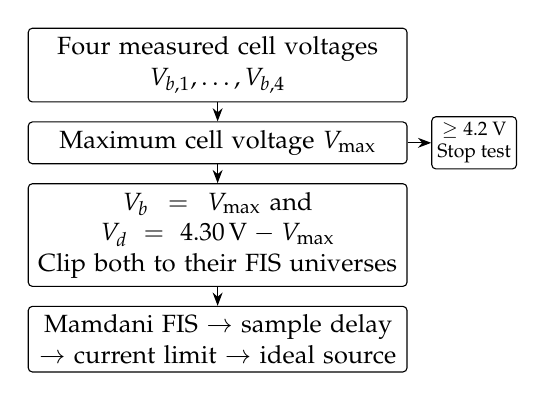
\begin{tikzpicture}[font=\small,>=Stealth,
 block/.style={draw,rounded corners=1.5pt,align=center,text width=4.6cm,inner sep=3pt},
 node distance=2.4mm]
\node[block] (cells) {Four measured cell voltages\\$V_{b,1},\ldots,V_{b,4}$};
\node[block,below=of cells] (max) {Maximum cell voltage $V_{\max}$};
\node[block,below=of max] (margin) {$V_b=V_{\max}$ and $V_d=4.30\,\mathrm{V}-V_{\max}$\\Clip both to their FIS universes};
\node[block,below=of margin] (fis) {Mamdani FIS $\rightarrow$ sample delay\\$\rightarrow$ current limit $\rightarrow$ ideal source};
\draw[->] (cells) -- (max);
\draw[->] (max) -- (margin);
\draw[->] (margin) -- (fis);
\node[draw,rounded corners=1.5pt,right=3mm of max,font=\scriptsize,align=center,inner sep=2pt] (stop) {$\ge4.2$ V\\Stop test};
\draw[->] (max) -- (stop);
\end{tikzpicture}
\caption{Signal paths in the Mamdani benchmark. The branch to the voltage event uses the maximum cell voltage directly.}
\label{fig:architecture}
\end{figure}

\subsection{Numerical settings and cases}
Table~\ref{tab:solver} describes the nominal runs. The refined solver check holds the electrical and controller periods at $1\,\mathrm{s}$, uses a $0.25\,\mathrm{s}$ maximum step, and sets the relative and absolute tolerances to $10^{-6}$ and $10^{-8}$. A separate check explicitly sets the SPS \texttt{powergui} time step and the Mamdani command period to $0.5\,\mathrm{s}$, uses a $0.25\,\mathrm{s}$ maximum step, and retains the nominal tolerances. Electrical updates at half-second time hits were verified from the logged cell voltages.

\begin{table}[htbp]
\centering\small
\caption{Numerical settings for nominal runs.}
\label{tab:solver}
\begin{tabular}{@{}p{0.44\columnwidth}p{0.48\columnwidth}@{}}
\toprule
Parameter & Setting\\
\midrule
Software & MATLAB/Simulink R2023b, Update 11\\
Global solver & Variable-step \texttt{ode23tb}\\
Step sizes & Initial and minimum automatic, maximum $1\,\mathrm{s}$\\
Tolerances & Relative $10^{-5}$ and absolute $10^{-7}$, autoscaling enabled\\
Electrical network & Discrete SPS \texttt{powergui}, $1\,\mathrm{s}$, Tustin/backward Euler\\
Mamdani command & $1\,\mathrm{s}$ update and one-sample delay, 101 centroid points\\
Voltage event & Sampled comparison $V_{\max}\ge4.2\,\mathrm{V}$\\
Additional stops & $99\,\%$ maximum cell SOC or $10{,}000\,\mathrm{s}$\\
\bottomrule
\end{tabular}
\end{table}

The compiled model reports a fixed-in-minor-step rate, $[0,1]$, for the maximum-voltage signal and the signal-dependent FIS evaluation. The unit delay and limiter implement the discrete command rate $[1,0]$ in the nominal runs. The voltage crossing occurred on the electrical sampling grid in every run. With solver refinement, intervening logged major steps retain the preceding maximum cell voltage. The thermal integrator is continuous. The configuration exports include the compiled rates and the local zero-crossing settings~\cite{mathworks_sample}.

The nominal comparison uses a $2.2\,\mathrm{A}$ ceiling and uniform initial SOC of $2.5\,\%$. The current-limit sweep repeats that condition with ceilings of $1.1$, $1.5$, and $1.8\,\mathrm{A}$. The mean-SOC sweep uses uniform initial values of $2.5$, $20$, and $40\,\%$. The imbalance sweep holds the mean at $20\,\%$ and varies the initial spread from 0 to 10 and 30 percentage points. The $30$-point case is repeated in reversed cell order to check dependence on pack ordering.

A separate output-range test uses the nominal $[0.5,2.2]$\,A FIS and the $[0.5,1.8]$\,A variant, both at a downstream current ceiling of $2.2$\,A. Each FIS is tested with uniform SOC at $2.5\%$, uniform SOC at $20\%$, and the ordered profile $(5,15,25,35)\%$ in BV1--BV4. The last two cases share the same initial mean and isolate the effect of a 30-percentage-point spread. The voltage stop, solver, sample periods, and model parameters are the same in each pair.

The extended runs use the nominal Mamdani FIS, a uniform $2.5\%$ initial SOC, and the $2.2$\,A current ceiling. Their voltage stop is disabled to characterize heating and the current and SOC trajectories after the common electrical event. They end at the SOC ceiling or time limit. The comparison of time to threshold uses the runs with the voltage stop enabled. For the nominal cases, a second endpoint is defined as the first logged sample at which the common cell SOC reaches $90\,\%$. This endpoint is reached before the voltage stop for both methods. The reported thermal rise is the maximum from the start up to that sample.

\subsection{Thermal estimation}
\label{sec:thermalmodel}
The estimated mean cell temperature $T$ obeys
\begin{equation}
C_{\mathrm{th}}\frac{dT}{dt}=I_{\mathrm{ch}}^{2}R_0-\frac{T-T_{\mathrm{amb}}}{R_{\mathrm{th}}}.
\label{eq:thermal}
\end{equation}
The ambient and initial temperatures are $25\,^\circ\mathrm{C}$. The thermal model is driven by measured simulated current and does not feed back into the electrical model. For constant $I$ and $T(0)=T_{\mathrm{amb}}$,
\begin{equation}
T(t)-T_{\mathrm{amb}}=I^2R_0R_{\mathrm{th}}\bigl(1-e^{-t/(R_{\mathrm{th}}C_{\mathrm{th}})}\bigr).
\label{eq:thermalcc}
\end{equation}
With $C_{\mathrm{th}}=40.5\,\mathrm{J/K}$ and $R_{\mathrm{th}}=20\,\mathrm{K/W}$, the time constant is $810\,\mathrm{s}$. The capacitance combines the approximate Eisto cell mass of $44\,\mathrm{g}$ with an assumed specific heat of $0.92\,\mathrm{J/(g\,K)}$, consistent with calorimetric measurements on another commercial 18650 LiCoO$_2$ cell~\cite{eisto2200,spinner2015}. The range $36$--$50\,\mathrm{J/K}$ represents about $0.82$--$1.14\,\mathrm{J/(g\,K)}$ at that mass.

The heat-loss resistance is an assumed boundary condition. Approximating the exposed cell as a cylinder with $18.4\,\mathrm{mm}$ diameter and $65.2\,\mathrm{mm}$ length gives an area of about $4.30\times10^{-3}\,\mathrm{m^2}$. The tested $10$--$30\,\mathrm{K/W}$ range corresponds to effective heat-transfer coefficients of about $8$--$23\,\mathrm{W/(m^2\,K)}$ when the full area is exposed and $R_{\mathrm{th}}=1/(hA)$. This parametric range tests cooling sensitivity without assuming a particular pack enclosure. Equation~\eqref{eq:thermal} accounts for ohmic heating and lumped cooling. Electrochemical heat, thermal gradients, and cell-to-cell heat transfer are outside this estimate.

\section{Mamdani controller}
\label{sec:fuzzy}
\subsection{Inputs and membership functions}
The voltage feedback is $V_b=V_{\max}$, with margin $V_d=4.30\,\mathrm{V}-V_b$. The internal $4.30\,\mathrm{V}$ reference defines the FIS coordinate and the original rule domains. The independent event in Eq.~\eqref{eq:events} governs the comparative run. FIS inputs are clipped to their respective ranges in Table~\ref{tab:mf}.

Each variable has five ordered triangular labels: very small (VS), small (S), medium (M), large (L), and very large (VL). The output membership functions were obtained by applying $I'=0.5+(I-0.5)(1.7/1.9)$ to the vertices of the original $[0.5,2.4]\,\mathrm{A}$ partition. This preserves their relative geometry and produces the nominal $[0.5,2.2]\,\mathrm{A}$ FIS used in the strategy comparisons and thermal analysis.

\begin{table*}[t]
\centering\small
\caption{Triangular membership vertices $(a,b,c)$ used by the FIS. Output vertices are rounded for display. The executable FIS contains the full-precision coefficients used in the calculation.}
\label{tab:mf}
\begin{tabular}{@{}lccc@{}}
\toprule
Label & $V_b$ (V) & $V_d$ (V) & $I_{\mathrm{FIS}}$ (A)\\
Universe & $[3.08,4.30]$ & $[0,1.22]$ & $[0.5,2.2]$\\
\midrule
\OutputMFs
\bottomrule
\end{tabular}
\end{table*}

Within each variable's universe, the same definition applies to antecedent and consequent sets:
\begin{equation}
\mu(x;a,b,c)=
\begin{cases}
1, & x=b,\\
(x-a)/(b-a), & a<x<b,\\
(c-x)/(c-b), & b<x<c,\\
0, & \text{elsewhere}.
\end{cases}
\label{eq:triangle}
\end{equation}
The slopes on nonzero-length segments are $1/(b-a)$ and $-1/(c-b)$. Adjacent labels overlap where their positive supports intersect within the universe. For example, the output VS and S sets overlap between approximately $0.7684$ and $1.1263\,\mathrm{A}$. The outer input sets use coincident vertices at the boundary. Some output vertices lie beyond the universe. The centroid uses only points within $[0.5,2.2]\,\mathrm{A}$. Figure~\ref{fig:mfs} shows the three partitions exported from the nominal FIS. For the output-range test, every output vertex $u$ is mapped to $0.5+(u-0.5)(1.3/1.7)$, including vertices outside the nominal universe. This preserves the relative positions and overlaps of the output sets. The input membership functions, rule base, and 101-point centroid discretization are identical in both FIS configurations. Figure~\ref{fig:membership_variant} shows the resulting output partition.

\begin{figure*}[t]
\centering
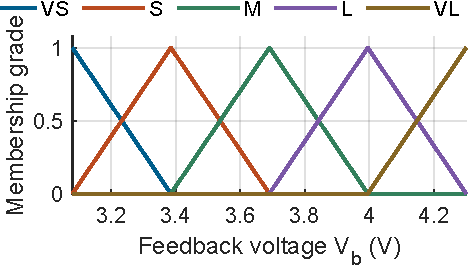
\includegraphics[width=.325\textwidth]{membership_vb.pdf}\hfill
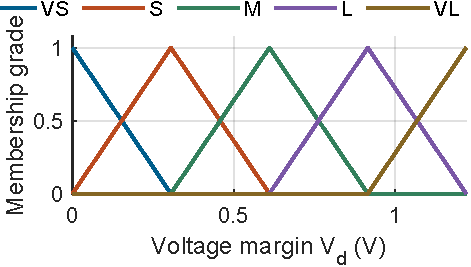
\includegraphics[width=.325\textwidth]{membership_vd.pdf}\hfill
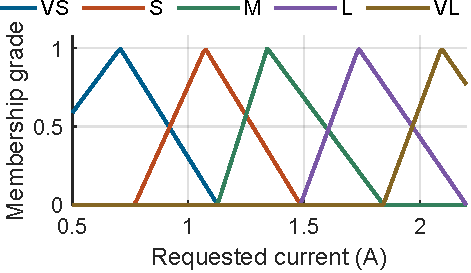
\includegraphics[width=.325\textwidth]{membership_current.pdf}
\caption{Triangular membership functions exported from the nominal FIS. Left to right, feedback voltage, voltage margin, and requested current.}
\label{fig:mfs}
\end{figure*}

\subsection{Rule base and centroid}
The Chuang et al.~\cite{chuang} rule policy uses $V_b$ categories as rows and $V_d$ categories as columns (Table~\ref{tab:rules}). If $i,j\in\{1,\ldots,5\}$ are the respective label indices, the consequent index is
\begin{equation}
q_{ij}=\begin{cases}
1,&j=1,\\
\min(5,j+1),&i\le3,\ j\ge2,\\
j,&i\ge4,\ j\ge2.
\end{cases}
\label{eq:rules}
\end{equation}
A very small margin selects the lowest current category in all five rows. Low-to-intermediate voltage rows promote the three intermediate margin categories (nine rules). High voltage rows keep the direct category mapping (six rules). The largest margin selects VL in all five rows. These four groups account for all 25 rules. The matrix is nondecreasing across each row and nonincreasing down each column. The resulting current is also shaped by set overlap and centroid inference.

\begin{table}[htbp]
\centering\small
\caption{Adopted Mamdani rule matrix~\cite{chuang}. Rows are feedback voltage $V_b$. Columns are voltage margin $V_d$.}
\label{tab:rules}
\begin{tabular}{@{}lccccc@{}}
\toprule
$V_b\backslash V_d$ & VS & S & M & L & VL\\
\midrule
VS & VS & M & L & VL & VL\\
S  & VS & M & L & VL & VL\\
M  & VS & M & L & VL & VL\\
L  & VS & S & M & L  & VL\\
VL & VS & S & M & L  & VL\\
\bottomrule
\end{tabular}
\end{table}

The rule weights are unity. For each rule, the AND operator and implication use minimum. Aggregation uses maximum:
\begin{align}
\alpha_{ij}&=\min[\mu_{A_i}(V_b),\mu_{B_j}(V_d)],\\
\mu_{\mathrm{agg}}(I)&=\max_{i,j}\min[\alpha_{ij},\mu_{C_{q_{ij}}}(I)] .
\end{align}
The centroid is the ratio of the first moment of $\mu_{\mathrm{agg}}$ to its area over the output universe, when the area is positive. The block evaluates this using 101 equally spaced output samples. The FIS specifies maximum for OR, while the adopted rules use only AND. For the static test at $(V_b,V_d)=(3.4,0.45)\,\mathrm{V}$, rules 7, 8, 12, and 13 contribute consequents M, L, M, and L. MATLAB gives a centroid of \StaticCurrent\,A (Fig.~\ref{fig:centroid}).

\begin{figure}[htbp]
\centering
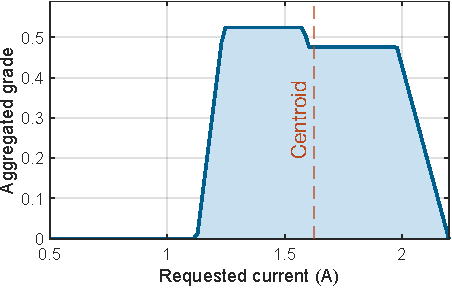
\includegraphics[width=.96\linewidth]{fis_centroid.pdf}
\caption{Aggregated consequent for the static test at $V_b=3.4\,\mathrm{V}$ and $V_d=0.45\,\mathrm{V}$. The dashed line locates the computed centroid.}
\label{fig:centroid}
\end{figure}

\subsection{Operating trajectory}
The two input coordinates can vary independently on the static map in Fig.~\ref{fig:surface}. In closed-loop operation their unclipped values follow $V_d=4.30\,\mathrm{V}-V_b$ and the limits on both inputs determine the endpoints. The decline in voltage margin generally lowers the request. The current also contributes to the measured terminal voltage. With internal state held fixed, the model's $R_0=0.016818\,\Omega$ gives about $16.8\,\mathrm{mV}$ of ohmic voltage change per ampere. Polarization and SOC account for additional voltage evolution.

\begin{figure}[htbp]
\centering
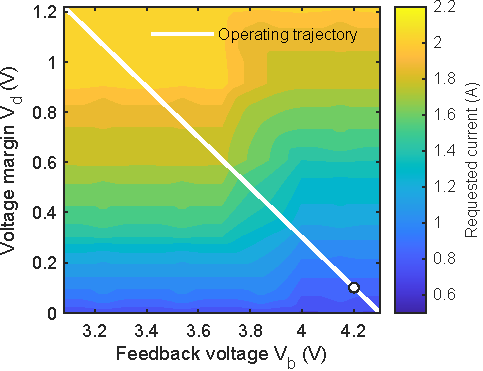
\includegraphics[width=.96\linewidth]{fis_surface.pdf}
\caption{Requested current surface for the FIS. The color scale gives current in amperes. The white line indicates the operating trajectory within the input ranges. The marker identifies the $4.2\,\mathrm{V}$ benchmark threshold.}
\label{fig:surface}
\end{figure}

\section{Results and discussion}
\label{sec:results}
\subsection{Electrical comparison with the Eisto charge profile}
\label{sec:eisto_comparison}
The Eisto charge profile provides an external reference for the electrical response of the battery model used in the benchmark. The datasheet specifies a $25\,^{\circ}\mathrm{C}$ CC--CV test at $1.1\,\mathrm{A}$ with a $4.2\,\mathrm{V}$ CV setpoint~\cite{eisto2200}. The simulation used the benchmark battery parameters, the same current and voltage settings, and a zero initial SOC in all four identical cells. It ran for $10{,}000\,\mathrm{s}$.

Voltage, current, and capacity were digitized on the published time axis. The datasheet current was converted from C-rate using the nominal capacity of $2.2\,\mathrm{Ah}$. The published capacity trace was normalized over its recorded span for comparison with simulated SOC on a shared 0--100\% scale (Fig.~\ref{fig:eisto_comparison}). The datasheet does not report absolute initial SOC. The simulated signals were interpolated at the digitized times up to about $155.4\,\mathrm{min}$, with the origin anchor excluded from the error calculation.

\begin{figure}[H]
\centering
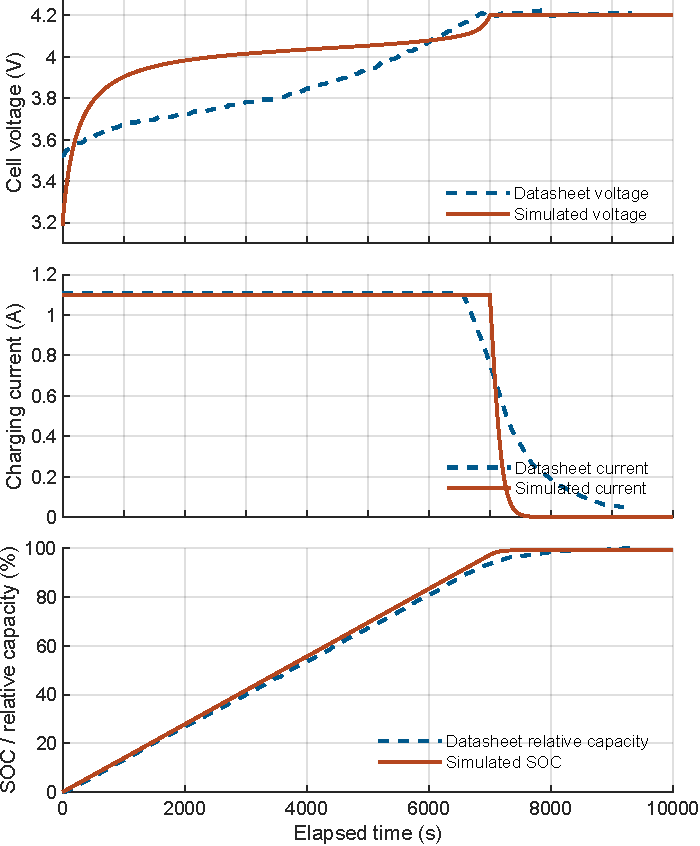
\includegraphics[width=.96\linewidth]{eisto_comparison.pdf}
\caption{Eisto charge profile~\cite{eisto2200} and simulated CC--CV response at $1.1\,\mathrm{A}$. The first sustained $4.2\,\mathrm{V}$ crossing occurs at \EistoRefV\,min in the datasheet and \EistoSimV\,min in the simulation.}
\label{fig:eisto_comparison}
\end{figure}

{\clubpenalty=10000 The first sustained crossing of $4.2\,\mathrm{V}$ occurred at approximately \EistoRefV\,min in the datasheet and \EistoSimV\,min in the simulation, a difference of \EistoAbsGapV\,min. Sustained events were identified at the first sample that met the criterion for at least $30\,\mathrm{s}$. For current taper, the criterion was a fall to $99\,\%$ of the CC level or below. The taper began at \EistoRefI\,min in the datasheet and \EistoSimI\,min in the simulation. The mean absolute errors were \EistoVoltMAE\,mV for voltage, \EistoCurrentMAE\,mA for current, and \EistoProgressMAE\ percentage points for SOC relative to normalized capacity. The model reproduced the voltage-crossing time more closely than the onset of the current taper. These discrepancies characterize the model's agreement with this published test and provide context for the comparison of the charging strategies below.\par}

\subsection{Nominal comparison and source tracking}
Figure~\ref{fig:nominal} shows the maximum cell voltage and applied current. With an identical initial state for all cells, each strategy gives equal cell voltages within the model. The Mamdani case took \ExtraTimeFZ\,s longer to reach the threshold, an increase of \RelativeExtraFZ\% relative to the CC--CV time \TimeCC\,s. It reached the same voltage event at a higher mean model SOC (Table~\ref{tab:nominal}), consistent with the smaller resistive contribution under lower current near the event. The times describe the approach to a voltage threshold. The charge delivered by that time differs between the strategies.

\begin{table}[htbp]
\centering\small
\caption{Nominal results up to the first crossing. Peak current and temperature rise are measured over the run up to and including the event.}
\label{tab:nominal}
\begin{tabular}{@{}lrrrr@{}}
\toprule
Strategy & $t_{4.2}$ (s) & $I_{\mathrm{pk}}$ (A) & SOC (\%) & $\Delta T_{\mathrm{pk}}$ (K)\\
\midrule
\NominalRows
\bottomrule
\end{tabular}
\end{table}

\begin{figure}[htbp]
\centering
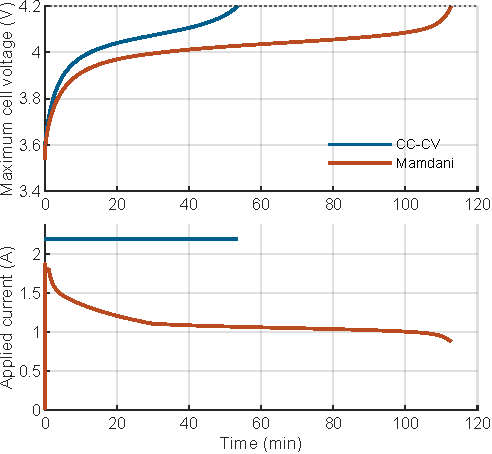
\includegraphics[width=.96\linewidth]{nominal_response.pdf}
\caption{Nominal comparison at $2.5\,\%$ initial SOC. Both traces end at the first sampled $4.2\,\mathrm{V}$ crossing.}
\label{fig:nominal}
\end{figure}

The nominal Mamdani applied peak is \PeakIFZ\,A under the common $2.2\,\mathrm{A}$ ceiling. Figure~\ref{fig:tracking} shows the initial zero command and the one-sample delay between inference and the source command. The maximum absolute error between the applied current magnitude and the delayed, limited command is \TrackingError\,A at the logged samples in this run. The CC stage tracks its setpoint to within $3\times10^{-6}\,\mathrm{A}$ at the logged nominal samples. The common ceiling and different applied current profiles must both be considered when interpreting the thermal and voltage results.

\begin{figure}[htbp]
\centering
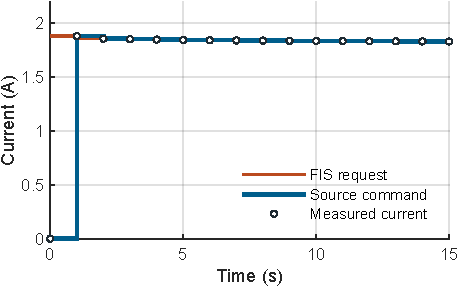
\includegraphics[width=.96\linewidth]{source_tracking.pdf}
\caption{First 15 seconds of the nominal Mamdani run. The current measurement coincides with the delayed and limited command at the electrical samples.}
\label{fig:tracking}
\end{figure}

At the shared $90\,\%$ SOC endpoint, CC--CV reached the target in \TimeNinetyCC\,s and Mamdani in \TimeNinetyFZ\,s (Table~\ref{tab:equal_soc}). Mamdani took \LateNinety\% longer relative to CC--CV and produced a smaller estimated peak temperature rise up to that endpoint. The timing difference persists when comparing at the same modeled charge state.

\begin{table}[htbp]
\centering\small
\caption{Comparison at $90\,\%$ SOC, with a $2.2\,\mathrm{A}$ current ceiling and uniform $2.5\,\%$ initial SOC. The temperature rise is the peak up to the endpoint.}
\label{tab:equal_soc}
\begin{tabular}{@{}lrrr@{}}
\toprule
Strategy & Time (s) & $V_{\max}$ (V) & $\Delta T_{\mathrm{pk}}$ (K)\\
\midrule
CC--CV & \TimeNinetyCC & \VoltNinetyCC & \RiseNinetyCC\\
Mamdani & \TimeNinetyFZ & \VoltNinetyFZ & \RiseNinetyFZ\\
\bottomrule
\end{tabular}
\end{table}

\subsection{Sensitivity to current limit and initial SOC}
Table~\ref{tab:current} isolates the current limit while retaining the identical initial SOC and a fixed Mamdani rule base and partition. The Mamdani time is weakly sensitive to the highest two limit settings because its current request exceeds $1.8\,\mathrm{A}$ only briefly in the nominal case. At the common $1.1\,\mathrm{A}$ ceiling, the time difference is \LateLowCap\% relative to the CC--CV time at that limit, compared with \RelativeExtraFZ\% at $2.2\,\mathrm{A}$. All cells have equal voltages in these uniform cases.

\begin{table}[htbp]
\centering\small
\caption{Effect of the current ceiling with uniform $2.5\,\%$ initial SOC. All voltage spreads at the threshold are $0\,\mathrm{mV}$.}
\label{tab:current}
\begin{tabular}{@{}rrrr@{}}
\toprule
Limit (A) & CC--CV (s) & Mamdani (s) & Mamdani $I_{\mathrm{pk}}$ (A)\\
\midrule
\CurrentRows
\bottomrule
\end{tabular}
\end{table}

At a fixed $2.2\,\mathrm{A}$ limit, increasing the uniform initial SOC reduces the time to the voltage event for both strategies (Table~\ref{tab:soc}). At a fixed mean initial SOC of $20\,\%$, more initial spread advances the event and leaves a larger terminal-voltage spread. Reversing the $30$-point case exchanges the first cell to cross (BV4 to BV1) while preserving the reported times and voltage spreads. Figure~\ref{fig:imbalance} shows the four cell trajectories for the increasing-order $30$-point case.

\begin{table*}[t]
\centering\small
\caption{Initial-SOC sensitivity at a $2.2\,\mathrm{A}$ limit. Voltage spreads are evaluated at each strategy's first crossing. The last column gives the first cell for CC--CV and Mamdani, respectively.}
\label{tab:soc}
\begin{tabular}{@{}lrrrrl@{}}
\toprule
BV1--BV4 initial SOC (\%) & CC--CV (s) & Mamdani (s) & CC--CV $\Delta V$ (mV) & Mamdani $\Delta V$ (mV) & First cell\\
\midrule
\SOCRows
\bottomrule
\end{tabular}
\end{table*}

\begin{figure}[htbp]
\centering
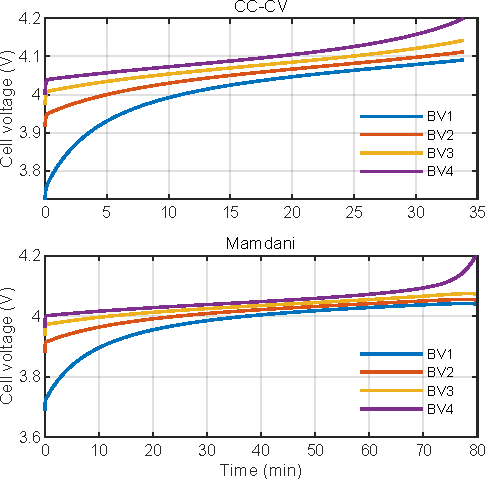
\includegraphics[width=.96\linewidth]{soc_imbalance.pdf}
\caption{Per-cell voltage for initial SOC values of 5, 15, 25, and $35\,\%$ in BV1--BV4. BV4 reaches the voltage threshold first in both cases.}
\label{fig:imbalance}
\end{figure}

For equal cell capacities $Q$ and charging efficiencies $\eta$, the shared current yields
\begin{equation}
\frac{d\,\mathrm{SOC}_k}{dt}
 = \frac{100\eta}{3600Q} I_{\mathrm{ch}}(t)
\end{equation}
for each cell's SOC in percent. Thus the initial SOC differences persist under these assumptions during common-current charging. Voltage spread can change as the cells progress along their nonlinear voltage characteristics. The values in Table~\ref{tab:soc} compare the pack state at each strategy's own stopping time.

\subsection{Sensitivity to the Mamdani output range}
Table~\ref{tab:output_sensitivity} compares both Mamdani configurations at their respective first $4.2$\,V crossings. Figure~\ref{fig:output_sensitivity} shows the maximum cell voltage and applied current on common axes for each initial SOC profile. This experiment reports electrical outcomes. The thermal comparisons in Tables~\ref{tab:equal_soc} and~\ref{tab:thermal} and Fig.~\ref{fig:extended} use the nominal $[0.5,2.2]$\,A FIS.

\begin{figure}[!t]
\centering
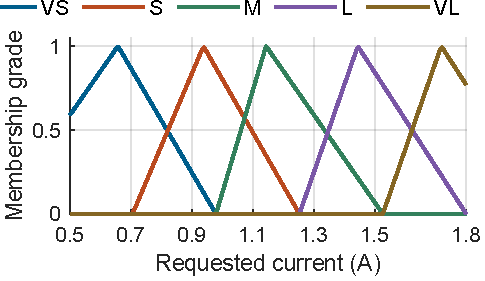
\includegraphics[width=.98\linewidth]{membership_current_180.pdf}
\caption{Output membership functions of the narrower Mamdani configuration, $[0.5,1.8]$\,A. All five sets are affinely rescaled from the nominal output partition.}
\label{fig:membership_variant}
\end{figure}

\begin{table*}[!t]
\centering\small
\caption{Mamdani output-range sensitivity at a fixed downstream ceiling of $2.2$\,A. $t_{4.2}$ is the time to the first sampled cell-voltage crossing, and $\Delta V$ is the inter-cell voltage spread at that crossing.}
\label{tab:output_sensitivity}
\begin{tabular}{lrrrr}
\toprule
& \multicolumn{2}{c}{$t_{4.2}$ (s)} & \multicolumn{2}{c}{$\Delta V$ (mV)}\\
\cmidrule(lr){2-3}\cmidrule(lr){4-5}
Initial SOC, BV1--BV4 (\%) & $[0.5,2.2]$ A & $[0.5,1.8]$ A & $[0.5,2.2]$ A & $[0.5,1.8]$ A\\
\midrule
\OutputSensitivityRows
\bottomrule
\end{tabular}
\end{table*}

\begin{figure*}[!t]
\centering
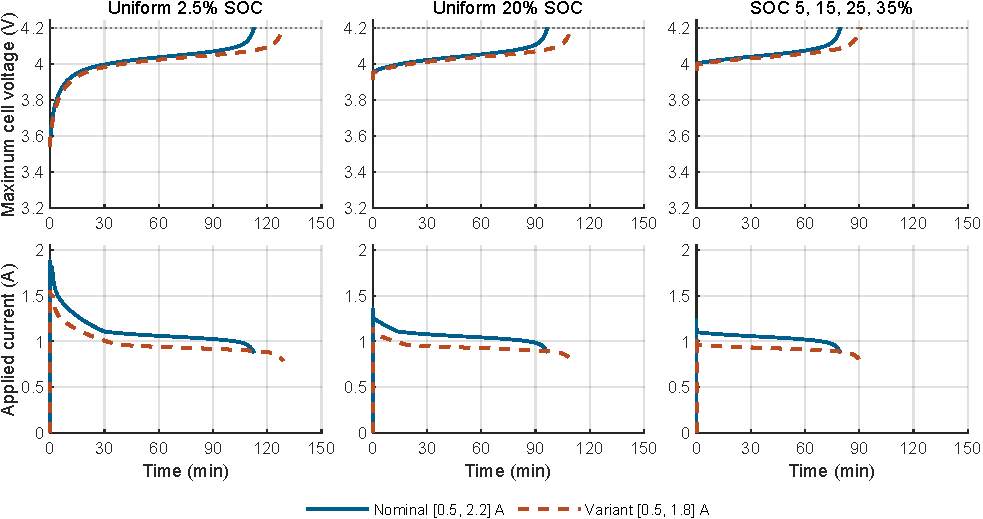
\includegraphics[width=.96\textwidth]{output_sensitivity.pdf}
\caption{Maximum cell voltage and applied current for the two Mamdani output ranges. Each column holds the initial SOC profile fixed. Each trace ends at its first sampled $4.2$\,V crossing.}
\label{fig:output_sensitivity}
\end{figure*}

Narrowing the output range changed $t_{4.2}$ by $\OutputDeltaBaseline$\,s at uniform $2.5\%$ SOC, $\OutputDeltaMean$\,s at uniform $20\%$ SOC, and $\OutputDeltaSpread$\,s with the same $20\%$ mean and a 30-point initial spread. The narrower partition delayed the crossing for all three profiles. At a fixed mean of $20\%$, the initial imbalance reduced the absolute delay attributable to the change in output range. The crossing spread remained zero in both uniform cases and increased slightly in the imbalanced case.

\subsection{Numerical checks}
Relative to the nominal settings, the finer solver changed $t_{4.2}$ by \CCSolverChange\,s for CC--CV and \FZSolverChange\,s for Mamdani. With the verified $0.5\,\mathrm{s}$ electrical and command periods, the first crossing was $0.5\,\mathrm{s}$ earlier for CC--CV and occurred at the same time for Mamdani. The strategy comparison was insensitive to these two refinements under the nominal conditions. The event used by the stop logic was checked against the logged maximum cell voltages in every comparative run.

\subsection{Extended trajectories and thermal estimates}
\label{sec:thermalresults}
In the nominal comparison, Eq.~\eqref{eq:thermalcc} gives about $1.60\,\mathrm{K}$ at the CC--CV crossing, consistent with the integrated temperature. In the extended CC--CV run the peak of \ExtendedCCPeak\,K occurred at \ExtendedCCPeakTime\,s, shortly after the transition. The nominal Mamdani rise peaked at \ExtendedFZPeak\,K at \ExtendedFZPeakTime\,s, before the voltage event. Cooling then exceeded ohmic heat generation for part of the continuing charge, as shown in Fig.~\ref{fig:extended}.

\begin{figure*}[t]
\centering
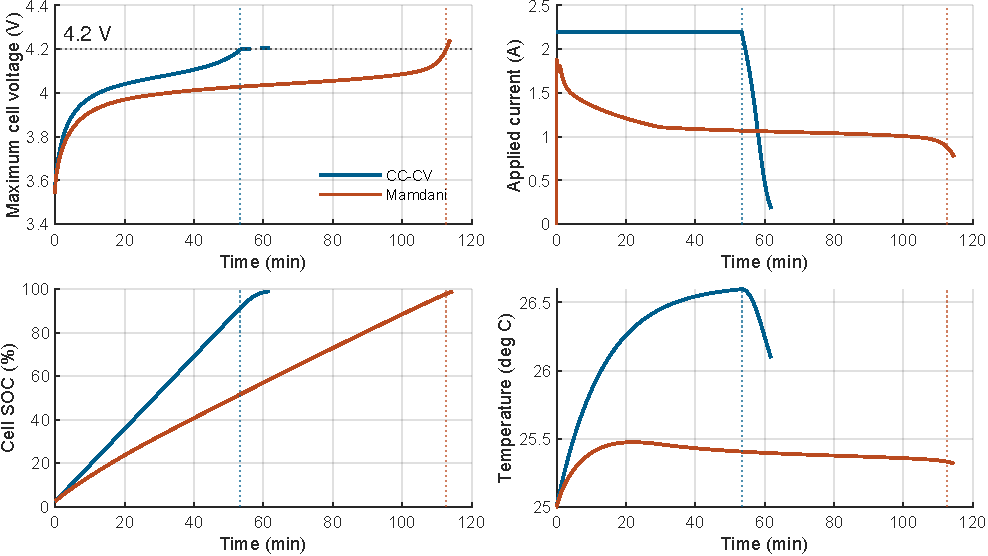
\includegraphics[width=.96\textwidth]{extended_response.pdf}
\caption{Extended runs from a uniform $2.5\%$ SOC, with a $2.2$\,A ceiling and the nominal Mamdani FIS. The dotted vertical lines mark each first crossing. In the voltage panel, dashed traces identify samples above $4.2\,\mathrm{V}$. These post-threshold portions are diagnostic.}
\label{fig:extended}
\end{figure*}

Both extended runs stopped at the $99\,\%$ SOC criterion, at \ExtendedCCStop\,s (CC--CV) and \ExtendedFZStop\,s (Mamdani). Maximum cell voltages were \ExtendedCCVoltage\,V and \ExtendedFZVoltage\,V, respectively. The CC--CV result includes the switching transient. The Mamdani trajectory continues under its internal reference with the voltage stop disabled. These excursions identify portions above the benchmark's $4.2\,\mathrm{V}$ threshold. They motivate using a separate voltage supervisor in the main comparison and in any subsequent implementation.

\begin{table}[htbp]
\centering\scriptsize
\caption{Thermal sensitivity in extended runs at a uniform initial SOC of $2.5\%$ and a $2.2$\,A current ceiling. Mamdani uses the nominal $[0.5,2.2]$\,A output range. $\Delta T$ is peak estimated rise and $t_{\mathrm{pk}}$ is its time. The first row gives the nominal setup.}
\label{tab:thermal}
\begin{tabular}{@{}rrrrrr@{}}
\toprule
 & & \multicolumn{2}{c}{CC--CV} & \multicolumn{2}{c}{Mamdani}\\
\cmidrule(lr){3-4}\cmidrule(l){5-6}
$C_{\mathrm{th}}$ & $R_{\mathrm{th}}$ & $\Delta T$ & $t_{\mathrm{pk}}$ & $\Delta T$ & $t_{\mathrm{pk}}$\\
(J/K) & (K/W) & (K) & (s) & (K) & (s)\\
\midrule
\ThermalRows
\bottomrule
\end{tabular}
\end{table}

The four parameter combinations in Table~\ref{tab:thermal} give peak rises of about $0.81$--$2.32\,\mathrm{K}$ for CC--CV and $0.27$--$0.65\,\mathrm{K}$ for Mamdani. Mamdani peaks earlier and at a lower rise in all four combinations. These differences reflect the current profiles under the common thermal model. They provide estimates of heating in the simulated conditions, with no inference of cell aging or life extension.

\subsection{Implementation limits and follow-up tests}
The ideal sources omit converter energy losses, bandwidth, current ripple, and voltage compliance. The observed ideal tracking therefore describes the simulation actuation. A real-time charging system would require characterization of converter response, sensing error, inference execution time, and latency from detecting an individual-cell limit to interrupting current. A BMS would need independent per-cell overvoltage and temperature supervision, an enforced current limit, and balancing suited to the expected cell mismatch~\cite{feng2019}. The studied maximum-voltage stop addresses a simulated threshold event. The voltage excursions in the extended runs illustrate why a pack-level setpoint or a fuzzy current request alone cannot establish all-cell compliance.

Follow-up work would use separate charge traces with specified initial SOC and repeat measurements at benchmark currents to assess whether the electrical agreement transfers beyond the manufacturer profile. Measured current and temperature transients would support thermal parameter identification. A model with actuator dynamics and subsequent real-time tests would quantify converter tracking and the BMS cutoff latency. Tests with cell-capacity and resistance mismatch would quantify the change in first-cell time and the effect of balancing.

\section{Conclusions}
Using the same $2.2\,\mathrm{A}$ ceiling and uniform initial SOC, CC--CV and Mamdani reached the first per-cell threshold in \TimeCC\ and \TimeFZ\,s. The time difference relative to CC--CV fell from \RelativeExtraFZ\% at $2.2\,\mathrm{A}$ to \LateLowCap\% at $1.1\,\mathrm{A}$. At the same $90\,\%$ SOC endpoint, the nominal Mamdani configuration also took longer and produced a lower estimated peak temperature rise. The thermal peak ordering persisted across the tested heat-capacity and thermal-resistance combinations. At $1.1\,\mathrm{A}$, the simulated first $4.2\,\mathrm{V}$ crossing differed by \EistoAbsGapV\,min from the Eisto reference. The voltage and current errors characterize agreement for this reported profile. The conclusions for the four-cell benchmark remain conditional on its battery model, ideal actuation, and prescribed thermal assumptions.

\section*{Computational materials}
The companion package contains both benchmark models, the nominal and narrower FIS files, the MATLAB entry point \texttt{run\_benchmark.m}, block configuration exports, and time-stamped signal CSVs. The entry point runs the benchmark and the Eisto comparison and regenerates the numerical tables and MATLAB figures. The readme lists the toolboxes, case IDs, and output locations.

\begin{thebibliography}{99}
\raggedright
\small
\setlength{\itemsep}{3pt}

\bibitem{chuang}
C.-C. Chuang, C.-J. Yao, and S.-T. Wu,
``Study on Fast Charging Method of Series Connected Lithium-Ion Battery Strings with Intelligent Control,''
in \textit{2020 International Conference on Fuzzy Theory and Its Applications (iFUZZY)}, Hsinchu, Taiwan, 2020, pp.~1--6, doi: \href{https://doi.org/10.1109/iFUZZY50310.2020.9297813}{10.1109/iFUZZY50310.2020.9297813}.


\bibitem{tomaszewska2019}
A. Tomaszewska \textit{et al.},
``Lithium-ion battery fast charging: A review,''
\textit{eTransportation},
vol. 1, Art. no. 100011, 2019,
doi: 10.1016/j.etran.2019.100011.

\bibitem{ghaeminezhad2022}
N. Ghaeminezhad and M. Monfared,
``Charging control strategies for lithium-ion
battery packs: Review and recent developments,''
\textit{IET Power Electronics},
vol. 15, no. 5, pp. 349--367, 2022,
doi: 10.1049/pel2.12219.

\bibitem{ali2018}
M. U. Ali, S. H. Nengroo, M. A. Khan,
K. Zeb, M. A. Kamran, and H.-J. Kim,
``A real-time Simulink interfaced fast-charging
methodology of lithium-ion batteries under
temperature feedback with fuzzy logic control,''
\textit{Energies},
vol. 11, no. 5, Art. no. 1122, 2018,
doi: 10.3390/en11051122.

\bibitem{karolyi2022}
G. Károlyi, A. I. Pózna, K. M. Hangos,
and A. Magyar,
``An optimized fuzzy controlled charging system
for lithium-ion batteries using a genetic
algorithm,''
\textit{Energies},
vol. 15, no. 2, Art. no. 481, 2022,
doi: 10.3390/en15020481.

\bibitem{nizam2022}
M. Nizam, H. Maghfiroh, A. Ubaidilah,
I. Inayati, and F. Adriyanto,
``Constant current-fuzzy logic algorithm
for lithium-ion battery charging,''
\textit{International Journal of Power
Electronics and Drive Systems},
vol. 13, no. 2, pp. 926--937, 2022,
doi: 10.11591/ijpeds.v13.i2.pp926-937.

\bibitem{feng2019}
F. Feng, X. Hu, J. Liu, X. Lin, and B. Liu,
``A review of equalization strategies for
series battery packs: Variables, objectives,
and algorithms,''
\textit{Renewable and Sustainable Energy Reviews},
vol. 116, Art. no. 109464, 2019,
doi: 10.1016/j.rser.2019.109464.

\balance
\bibitem{sardahi2026}
Y. Sardahi, A. Salem, and J. Farris,
``Current-stress-aware fuzzy logic control
for safe fast charging of lithium-ion
battery packs,''
\textit{Energies},
vol. 19, no. 17, Art. no. 3975, 2026,
published August 24, 2026, doi: \href{https://doi.org/10.3390/en19173975}{10.3390/en19173975}.

\bibitem{kalk2024}
A. Kalk, L. Leuthner, C. Kupper, and M. Hiller,
``An Aging-Optimized State-of-Charge-Controlled Multi-Stage Constant Current (MCC) Fast Charging Algorithm for Commercial Li-Ion Battery Based on Three-Electrode Measurements,''
\emph{Batteries}, vol.~10, no.~8, Art.~267, 2024,
doi: \href{https://doi.org/10.3390/batteries10080267}{10.3390/batteries10080267}.

\bibitem{perfil2024}
Manjunatha S, Rakesh K A, and A. K. Pratiwadibhayankaram,
``A Fast Charging Method for Lithium ion Batteries Based on a Unique Current Profile Method,''
\emph{SAE Technical Paper} 2024-26-0114, 2024,
doi: \href{https://doi.org/10.4271/2024-26-0114}{10.4271/2024-26-0114}.

\bibitem{eisto2200}
Shenzhen Eisto Electronics Co., Ltd., \emph{Specifications for the Cylindrical 18650-2200mAh Lithium-Ion Rechargeable Cell}, secs.~5--6 and p.~7. The cited copy specifies neither a publication date nor a revision identifier.
\href{https://www.eistoelectronics.com/web/userfiles/download/ICR18650-2200mAhBatteryDatasheet.pdf}{Manufacturer datasheet}.

\bibitem{spinner2015}
N. S. Spinner, R. Mazurick, A. Brandon, S. L. Rose-Pehrsson, and S. G. Tuttle,
``Analytical, numerical and experimental determination of thermophysical properties of commercial 18650 LiCoO$_2$ lithium-ion battery,''
\textit{Journal of The Electrochemical Society}, vol. 162, no. 14, pp. A2789--A2795, 2015,
doi: \href{https://doi.org/10.1149/2.0871514jes}{10.1149/2.0871514jes}.

\bibitem{mathworks_sps}
MathWorks, ``Controlled Current Source,'' \textit{Simscape Electrical Specialized Power Systems documentation}.
\href{https://www.mathworks.com/help/releases/R2023b/sps/powersys/ref/controlledcurrentsource.html}{R2023b documentation}.
\bibitem{mathworks_sample}
MathWorks, \emph{Types of Sample Time}, Simulink documentation.
\url{https://www.mathworks.com/help/simulink/ug/types-of-sample-time.html}

\end{thebibliography}
\end{document}

